\begin{ex}
(Fuvest) Um recenseamento revelou as seguintes características sobre a idade e a escolaridade da população de uma cidade:
 \begin{center}
   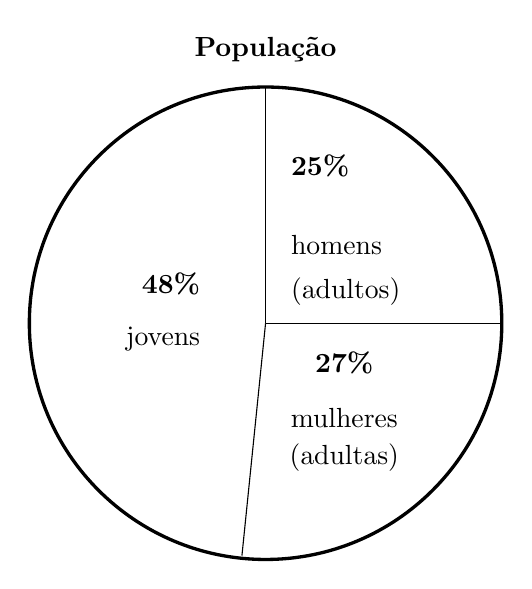
\begin{tikzpicture}
     \draw (15,0)[very thick] circle [radius = 3];
     \draw node at (15,3.2) [above] {\textbf{População}};
     \draw (15,0)--(18,0); \draw (15,0)--(15,3);\draw (15,0)--(14.7,-2.95);
     \node at (15.2,2) [right] {\textbf{25\%}};\node at (15.2,1) [right] {homens}; \node at (15.2,.4) [right] {(adultos)};\node at (16,-.5)  {\textbf{27\%}};
     \node at (16,-1.2) {mulheres};\node at (16,-1.7) {(adultas)};
     \node at (13.8,.5) {\textbf{48\%}};\node at (13.7,-.2) {jovens};
 \end{tikzpicture}

\end{center}
\begin{center}
   
   \begin{tabular}{|c|c|c|c|} \hline
    Escolaridade     & Jovens & Mulheres & Homens   \\ \hline
    Fundamental Incompleto  & 30\%    & 15\%   & 18\%  \\ \hline
    Fundamental Completo  & 20\%     & 30\%   &  28\%   \\  \hline
    Médio Incompleto  &  26\%  &  20\%  & 16\%  \\  \hline
    Médio Completo  &  18\%  &  28\%  &  28\%  \\  \hline
    Superior Incompleto & 4\%  &  4\%  &  5\%  \\  \hline
    Superior Completo & 2\%  & 3\%  & 5\%  \\   \hline
   \end{tabular}
\end{center}

Se for sorteada ao acaso uma pessoa da cidade, a probabilidade de ela ter curso superior ( completo ou incompleto) é:
   \begin{enumerate}[(a)]
   \item 6,12\%
   \item 7,27\%
   \item 8,45\%
   \item 9,57\%
   \item 10,23\%
   \end{enumerate}

  \begin{sol}
   resposta: b \\
   6\% de 48\% (jovens) ; 7\% de 27\% (mulheres); 10\% de 25\% (homens) \\
   $0,06\cdot0,48+0,07\cdot0,27+0,10\cdot0,25=0,0727=7,27\%$
   \end{sol}
\end{ex}